
\documentclass{amsart}

\usepackage[numbers]{natbib}
 \usepackage{epsfig}
 \usepackage{tikz}

\usepackage{graphicx,fancybox,amssymb,color,amsmath,amssymb,amsthm,amsfonts,pgf}
\usepackage{fancybox,graphicx,dsfont,pgf}
\usepackage{amsmath,amsthm,amsfonts,amssymb,fancybox,float}
\usepackage{subfigure,color,wrapfig}

\usepackage{latexsym}

\usepackage{dsfont}

\newtheorem{theorem}{Theorem}[section]
\newtheorem{corollary}[theorem]{Corollary}

\newtheorem{lemma}[theorem]{Lemma}
\newtheorem{proposition}[theorem]{Proposition}
\newtheorem{question}{Question}[section]
\newtheorem{exercise}{Exercise}[section]
\newtheorem{conjecture}{Conjecture}[section]
\theoremstyle{definition}
\newtheorem{definition}[theorem]{Definition}
\theoremstyle{remark}
\newtheorem{remark}[theorem]{Remark}
\theoremstyle{remark}
\newtheorem{example}{Example}[section]
\theoremstyle{definition}
\newtheorem{puzzler}{Pytek}

\numberwithin{equation}{section}

\usepackage{color,soul}

\title[ASEP and Quadratic Harnesses]{Asymmetric Simple Exclusion Process  with open boundaries and Quadratic Harnesses }

\author{
W{\l}odek  Bryc
}

\address{
Department of Mathematics,
University of Cincinnati,
PO Box 210025,
Cincinnati, OH 45221--0025, USA}
\email{Wlodzimierz.Bryc@UC.edu}

\author{Jacek Weso{\l}owski}
\address{ Faculty of Mathematics and Information Science
Warsaw University of Technology pl. Politechniki 1 00-661
Warszawa, Poland}
\email{wesolo@alpha.mini.pw.edu.pl}

\keywords{Exclusion process with open boundary;Markov processes;Large deviations;Askey-Wilson
distribution;quadratic harness}
\subjclass[2000]{60K35,82C22}

\date{Created: July 2015. Version {\tt \jobname.tex}. Printed \today}

\begin{document}
\maketitle
\begin{abstract}
We establish a correspondence   between a family of Markov processes called
quadratic harnesses and a family of finite state asymmetric exclusion processes   with open boundaries.   As  applications, we give a quick proof of
the large deviations principle  for the total number of particles in the system,   and 
show how  explicit formulas for the average occupancy of a site arise for special choices of parameters.
\end{abstract}

\section{Introduction}
\subsection{Asymmetric simple exclusion process with open boundaries}
Asymmetric simple exclusion process (ASEP) is a Markov model for  random particles that cannot occupy the same position, and tend to move to the adjacent site with the rate that is larger to the
right   than to the left.
There are several versions of the model; for example, \citet{spitzer1970interaction} considers ASEP on the infinite number and the finite number of sites.  In this paper
we are interested in a particle system on a finite lattice of $N\geq 2$ points $S=\{1,\dots,N\}$,
 where each site $j\in S$ can have only $\tau_j=0$ or $\tau_j=1$ particles. The term ``open boundary''
refers to the fact that particles can be inserted and removed from both boundary points.
This version of ASEP was extensively studied in physics,
  see e.g. \cite{bertini2002macroscopic,blythe2000exact,derrida1992exact,derrida2004current,derrida1993exact,derrida2001free,derrida2002exact}. Survey \citet{blythe2007nonequilibrium} gives additional references and motivation.

  An informal description of the exclusion process is that particles are placed at rate $\alpha>0$
in position $1$, and at rate $\delta\geq 0$ in position $N$, provided the location is empty. Particles are also removed at rate $\gamma\geq 0$  from
location $1$ and removed  at rate $\beta>0$ from  site $N$.
Particles attempt to move to the nearest neighbor; to the right with rate 1 and to the left with rate $q\geq 0$; however they cannot move if the neighbor site is already occupied.
 Parameters $\alpha,\beta,\gamma,\delta$ describe behavior at the boundaries; parameter $q$ determines the degree of asymmetry, see Fig. \ref{Fig1}.
 Exclusion process is symmetric, when
 $q=1$; the case $q>1$ is similar to  $q<1$ due to ``particles-holes duality'', see e.g. discussion of this  point in
 \cite{uchiyama2004asymmetric}.  Throughout this paper we will assume that $q<1$.

\begin{figure}[H]
  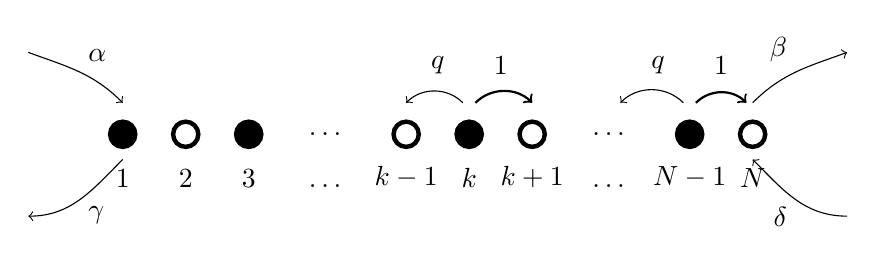
\begin{tikzpicture}[scale=.8]
 
\draw [fill=black, ultra thick] (.5,1) circle [radius=0.2];
\draw [fill=black, ultra thick] (2.5,1) circle [radius=0.2];
  \draw [ultra thick] (1.5,1) circle [radius=0.2];

 
  \draw [ultra thick] (5,1) circle [radius=0.2];
   \draw [fill=black, ultra thick] (6,1) circle [radius=0.2];

    \draw [ultra thick] (7,1) circle [radius=0.2];

      \draw [fill=black, ultra thick] (9.5,1) circle [radius=0.2];
   \draw [ultra thick] (10.5,1) circle [radius=0.2];

        \draw[->] (-1,2.3) to [out=-20,in=135] (.5,1.5);
   \node [above right] at (-.2,2) {$\alpha$};
     \draw[->] (10.5,1.5) to [out=45,in=200] (12,2.3);
     \node [above left] at (11.2,2) {$\beta$};

                 \node  at (8.25,1) {$\dots$};  \node  at (3.75,1) {$\dots$};
           \node [above] at (6.5,1.8) {$1$};
      \draw[->,thick] (6.1,1.5) to [out=45,in=135] (7,1.5);
        \node [above] at (5.5,1.8) {$q$};
            \draw[<-] (5,1.5) to [out=45,in=135] (5.9,1.5);

                                  \node [above] at (10,1.8) {$1$};
                \draw[->,thick] (9.6,1.5) to [out=45,in=135] (10.4,1.5);
               \node [above] at (9,1.8) {$q$};

                 \draw[<-] (8.4,1.5) to [out=45,in=135] (9.4,1.5);
      

       \draw[<-] (-1,-.3) to [out=0,in=-135] (.5,0.6);
   \node [below right] at (-.2,0) {$\gamma$};

        \draw[<-] (10.5,.6) to [out=-45,in=180] (12,-.3);
   \node [below left] at (11.2,0) {$\delta$};

       \node [above] at (0.5,0) {$1$};
    \node [above] at (1.5,0) {$2$};
   \node [above] at (2.5,0) {$3$};
     \node [above] at (3.75,0) {$\dots$};

   \node [above] at (5,0) {$k-1$};
     \node [above] at (6,0) {$k$};
       \node [above] at (7,0) {$k+1$};
        \node [above] at (8.25,0) {$\dots$};
         \node [above] at (10.5,0) {$N$};
          \node [above] at (9.5,0) {$N-1$};
\end{tikzpicture}
\caption{Asymmetric Simple Exclusion process with open boundary and  parameters $\alpha,\beta,\gamma,\delta, q$.
Black disks represent occupied sites. \label{Fig1}}
\end{figure}

Time evolution of such a system is described by a continuous time Markov process $(\tau_1(t),\dots,\tau_N(t))$ with finite state space  $\{0,1\}^N$, see e.g. \cite[Fromulas (2.1)-(2.3)]{sandow1994partially}.
We do not provide the details,
 as we are interested only in the (unique) invariant probability measure $\pi_N$ of the Markov chain $(\tau_1(t),\dots,\tau_N(t))$.
 Using the notation borrowed from statistical physics, by $\langle \cdot\rangle_N$
  we denote the average with respect to this  probability measure and  by $(\tau_1,\dots,\tau_N)\in\{0,1\}^N$ we denote
  the random vector with the invariant distribution $\pi_N$. For example, ${\langle}\tau_k{\rangle}_N$
  is the average occupancy of site $k$ with respect to $\pi_N$.

\subsection{Matrix solution}
The celebrated matrix method of \citet{derrida1993exact} introduces
a probability measure on $\{0,1\}^N$ using a pair  ${\mathbf{D}}$ and ${\mathbf{E}}$ of infinite matrices with ${\mathbf{D}}$ representing the occupied site, ${\mathbf{E}}$ representing an empty site, and a pair of vectors, where
  $\langle W|$ is a row vector and $|V\rangle$ is a column vector. We will denote this measure by $\pi_N$,
  as it will turn out to be the invariant measure discussed in the previous section.
  For our purposes it is convenient to recast the  expression from \cite{derrida1993exact}
   into the formula for the joint generating function
\begin{equation}
\label{MatrixSolution}
\left\langle \prod_{j=1}^N t_j^{\tau_j}\right\rangle_N=\frac{1}{K_N}\langle W| ({\mathbf{E}}+t_1{\mathbf{D}})({\mathbf{E}}+t_2{\mathbf{D}})\dots({\mathbf{E}}+t_N{\mathbf{D}})|V\rangle.
\end{equation}
Here
 \begin{equation}
   \label{KN}
   K_N=\langle W| ({\mathbf{E}}+ {\mathbf{D}})^N|V\rangle
 \end{equation} is the normalizing constant, which in the physics literature is
 called the partition function and  is usually denoted by letter $Z$; in this paper we need to reserve letter $Z$ for a Markov process that we  introduce in Section \ref{AMP}.

Note that   representation \eqref{MatrixSolution}   is valid only for $\<W|V{\rangle}\ne0$.  In ref. \cite{derrida1993exact} the authors verify  that $\langle \prod_{j=1}^N t_j^{\tau_j}\rangle_N$ is indeed the
moment generating function of the invariant
 distribution $\pi_N$ of the exclusion process with parameters $\alpha,\beta,\gamma,\delta, q$, provided that
   the matrices and the vectors satisfy relations
 \begin{eqnarray}
  {\mathbf{D}}{\mathbf{E}}-q{\mathbf{E}}{\mathbf{D}}&=&{\mathbf{D}}+{\mathbf{E}} ,\label{q-comm-Derrida}\\
\langle W|(\alpha {\mathbf{E}}-\gamma {\mathbf{D}})&=&\langle W| ,\label{W}\\
(\beta {\mathbf{D}}-\delta {\mathbf{E}})|V\rangle&=&|V\rangle. \label{V}
\end{eqnarray}
\citet{derrida1993exact} give a detailed proof   for the case when $q=0$, and sketch the proof for the general $q$.
\citet[Section III]{sandow1994partially}  proves the invariance of the probability
measure determined by \eqref{MatrixSolution} for arbitrary $q$.

Formula \eqref{MatrixSolution} offers the flexibility of choosing convenient vectors and matrices.
Refs. \cite{derrida1993exact,derrida2003exact,enaud2004large} \cite{sasamoto1999one} \cite{uchiyama2004asymmetric} show such choices for a suitable
 ranges of the parameters,
  and use the explicit representations to derive   properties of the ASEP.
One of our goals is to re-derive some of the properties of ASEP using a
completely different representation which is  in terms of certain Markov processes.

  We note that  \citet[page 1384]{essler1996representations} point out that  matrix solution cannot exist when $\alpha\beta=\gamma\delta$.
 They also point out the importance of a more general requirement $\alpha\beta-q^k\gamma\delta\ne0$ for $k=0,1,\dots$.
 Our Markov process representation requires additional restrictions on the parameters, which imply $\gamma\delta<\alpha\beta$.

\subsection{Auxiliary Markov process - quadratic harness}\label{AMP}
In this section we introduce an auxiliary Markov processes defined on another probability space
which is unrelated to the invariant measure described in \eqref{MatrixSolution}.
To make the distinction more transparent,
we denote by ${\mathds{E}}(X)$ the expected value of a random variable $X$ on this probability space. Our auxiliary Markov process is different than  the
 Markov process associated with ASEP  in \cite{corteel2007markov}, and the way the two processes are tied together is also different. However, there is a common thread of Askey-Wilson polynomials in the background.

\citet{Bryc-Wesolowski-08} use the orthogonality measures of Askey-Wilson polynomials to construct a (unique) Markov process $(Z_t)$ for
 parameters $A,B,C,D,q$ with the following properties:
 \begin{itemize}
   \item $(Z_t)$ has a sequence of orthogonal martingale polynomials $$\langle\mathbf{r}_t(x)|=[r_0(x;t), r_1(x;t),\dots],$$
    i.e.  $r_n(x;t)$ ($n=0,1,\dots$) is a polynomial of degree $n$ in variable $x$ such that:
    \begin{enumerate}
      \item $r_0(x;t)=1$;
      \item ${\mathds{E}}\left(r_n(Z_t;t)r_m(Z_t;t)\right)=0$ for $m\ne n$;
      \item ${\mathds{E}}(r_n(Z_t;t)|Z_s)={\mathds{E}}(r_n(Z_t;t)|\sigma(Z_v:v\leq s))=r_n(Z_s;s)$ for $s\leq t$.
    \end{enumerate}
    \item The Jacobi matrix of the orthogonal polynomials $\{r_n(\cdot;t)\}$ is a tridiagonal infinite matrix which
    depends linearly on parameter $t$. We will write it  as $t{\mathbf{x}}+{\mathbf{y}}$, and we will write the so called ``three step recurrence" in vector notation as
    \begin{equation}
      \label{three-step} x \langle\mathbf{r}_t(x)| = \langle\mathbf{r}_t(x)|(t{\mathbf{x}}+{\mathbf{y}}).
    \end{equation}
    This appears in  \cite[page 1244]{Bryc-Wesolowski-08}.
    \item The Jacobi matrix is determined uniquely from the $q$-commutation equation
    \begin{equation}
      \label{q-comm}
      {\mathbf{x}} {\mathbf{y}} - q {\mathbf{y}} {\mathbf{x}} ={\mathbf{I}}
    \end{equation}
    and the initial conditions  {}
    \begin{equation}
      \label{ini-cond}
      {\mathbf{x}}=\left[\begin{matrix}
        \gamma_0 & {\varepsilon}_1 & 0 &\dots \\
        \alpha_0 & & & \\
        0 & & & \\
        \vdots & & & \\
      \end{matrix}\right], \quad {\mathbf{y}}=\left[\begin{matrix}
        \delta_0 & \varphi_1 & 0 &\dots \\
        \beta_0 & & & \\
        0 & & & \\
        \vdots & & & \\
      \end{matrix}\right]\,,
    \end{equation}
    where $\alpha_0,\beta_0,\gamma_0,\delta_0,{\varepsilon}_1,\varphi_1$ depend on parameters $A,B,C,D,q$ through formulas in
    \cite[page 1243]{Bryc-Wesolowski-08}; these formulas are reproduced in the proof of Theorem \ref{T-rep} below, see e.g.
    \eqref{gamma0}.
 \end{itemize}
 The goal of \cite{Bryc-Wesolowski-08} was the construction of the so called quadratic harnesses, i.e., Markov processes $(Z_t)_{t\geq 0}$
 with harness property
 \begin{equation}\label{QH}
  {\mathds{E}}(Z_t|Z_s,Z_u)=\frac{u-t}{u-s}Z_s+\frac{t-s}{u-s}Z_u
 \end{equation}
 and quadratic conditional variances under a two-sided conditioning.

In general, parameters $A,B,C,D$ can be complex numbers, which need to satisfy appropriate constraints for the process $(Z_t)$ to exist. In this paper we
will only need real-valued parameters $A\geq 0,B\leq 0,C\geq 0,D\leq 0$, and $q\geq 0$.
 Specialized to this case, \cite[Theorem 1.2]{Bryc-Wesolowski-08} assures that Markov process $(Z_t)_{t\geq 0}$ is well defined under
 the following constraints on the parameters:
 \begin{equation}
   \label{contraints1}
   q<1, \quad    AC<1, \quad
       BD<1.
 \end{equation}
Some of these conditions have an interpretation in terms of an associated ASEP, see Remark \ref{Rem:interpret}.

\section{Representing  a matrix solution by the auxiliary Markov process}
We now return  to the study of invariant measure of ASEP with parameters $\alpha>0,\beta>0,\gamma\geq 0,\delta\geq 0,q\geq
0$. Our goal is to associate an appropriate process $(Z_t)$ with the ASEP. Denote
 \begin{eqnarray}
\kappa_{\pm}(\alpha,\gamma)&=&\frac{1-q-\alpha+\gamma\pm\sqrt{(1-q-\alpha+\gamma)^2+4\alpha \gamma}}{2\alpha} \,, \label{kappa1}\\
\kappa_{\pm}(\beta,\delta)&=&\frac{1-q-\beta+\delta+\sqrt{(1-q-\beta+\delta)^2+4\beta\delta}}{2\beta} \,. \label{kappa2}
\end{eqnarray}

 Let $(Z_t)_{t\geq 0}$ be the Markov process from Section \ref{AMP} with parameters {}
\begin{equation}
  \label{ABCD}
  A=\kappa_{+}(\beta,\delta), \; B= \kappa_{-}(\beta,\delta), \; C=\kappa_{+}(\alpha,\gamma),\;D=\kappa_{-}(\alpha,\gamma).
\end{equation}
Notice that $A,B,C,D$ are real, $ABCD=\gamma\delta/(\alpha\beta)$, and $A,C\geq 0$ while $B,D\leq 0$.

Our main result is the following representation of the joint generating function of the invariant measure of the ASEP in terms of the stochastic process $(Z_t)$ from Section \ref{AMP}.
\begin{theorem}
  \label{T-rep}
Suppose that the parameters of ASEP are such that conditions \eqref{contraints1} are satisfied for $A,B,C,D$ defined in
\eqref{ABCD}. Then for $0<t_1\leq t_2\leq \dots\leq t_N$ the joint generating function of the invariant measure of the ASEP  is
  \begin{equation}\label{QHsolution}
\left\langle \prod_{j=1}^N t_j^{\tau_j}\right\rangle_N=\frac{{\mathds{E}}\left(\prod_{j=1}^N(1+t_j+\sqrt{1-q}\,Z_{t_j})\right)}{{\mathds{E}}\left((2+\sqrt{1-q}\,Z_1)^N\right)}.
  \end{equation}
 \end{theorem}
Since the left hand side is a polynomial in $t_1,\dots,t_N$, it is clear that formula \eqref{QHsolution} determines $\langle \prod_{j=1}^N t_j^{\tau_j}\rangle_N$ completely.

The proof of Theorem \ref{T-rep} appears  in Section \ref{Sect:PTR}. We conclude this section with  remarks.
 \begin{remark}\label{Rem:interpret}
To discuss the constraints on the parameters, we first note that \eqref{contraints1} implies that
$$\frac{\gamma\delta}{\alpha\beta}=ABCD<1,$$
so that the obstacles \cite[page 1384]{essler1996representations} to the existence of a matrix representation are automatically
avoided. Condition $AC<1$ has natural physical interpretation -- in terminology of \cite{derrida2003exact}
 it identifies the ``fan region" of ASEP. Condition $BD<1$  seems to be technical, and we do not have its interpretation in terms of an
ASEP.
\end{remark}

\begin{remark}
Suppose that $(Z_t)$ is a Markov process from Section \ref{AMP} with $0\leq q<1$ and parameters $A,B,C,D$ that
  satisfy \eqref{contraints1}. If in addition
$(1+A)(1+B)>0$, $(1+C)(1+D)>0$, then the right hand side of \eqref{QHsolution} determines the invariant measure of an ASEP with
parameters
\begin{equation}
  \label{Jacek}
  \beta=\frac{1-q}{(1+A)(1+B)},
\; \alpha=\frac{1-q}{(1+C)(1+D)}, \; \gamma=\frac{-(1-q) CD}{(1+C)(1+D)}, \; \delta=\frac{-(1-q)AB}{(1+A)(1+B)}.
\end{equation}
\end{remark}

\begin{remark}
A special case of formula \eqref{QHsolution} relates $\<t^{\sum_{j=1}^n\tau_j}{\rangle}_N$ to the $N$-th moment of  $(1+t+\sqrt{1-q}Z_t)$, i.e. to the moments of an Askey-Wilson law.
The exact formula for the "partition function" ${\mathds{E}}(2+\sqrt{1-q}Z_1)^N$ has been known since \cite[Equation (57)]{blythe2000exact}.
    \citet[Theorem 1.3.1]{josuat2011combinatorics} generalizes this to the exact formula for the case when $\gamma=\delta=0$.
   A special case   $\alpha=\beta=1-q$ appeared earlier in \cite{josuat2011rook},
  and was related to combinatorics of permutations. For a more analytic approach, see  \cite{szablowski2015moments}.
Formulas for moments of  more general Askey-Wilson laws appear in
\cite{corteel2012formulae,kim2014moments}.

\end{remark}

\subsection{Proof of Theorem \ref{T-rep}}\label{Sect:PTR} {}
Our motivation and starting point is Ref. \cite{uchiyama2004asymmetric} which represents matrices ${\mathbf{E}},{\mathbf{D}}$
by the Jacobi matrices of the Askey-Wilson polynomials, with vectors $\langle W|=[1,0,0,\dots]$ and $|V\rangle=[1,0,0,\dots]^T$.
Ref. \cite{uchiyama2004asymmetric} then uses these matrices to give  the integral formulae for the partition function and for the $m$-point correlation function
$\langle \tau_{j_1}\tau_{j_2}\dots\tau_{j_m}\rangle$.
These integral formulas inspired our search for representation in terms of the quadratic harnesses.
Our starting point is a slight variation of \cite[formula (4.5)]{uchiyama2004asymmetric}. We use matrices ${\mathbf{x}}$, ${\mathbf{y}}$ from \eqref{three-step}   to rewrite the matrices in \eqref{MatrixSolution} as
\begin{equation}
  \label{J2C}
{\mathbf{E}}= \frac{1}{1-q}{\mathbf{I}}+\frac{1}{\sqrt{1-q}}\,{\mathbf{y}}, \quad {\mathbf{D}}=\frac{1}{1-q}{\mathbf{I}}+\frac{1}{\sqrt{1-q}}\,{\mathbf{x}}\,,
\end{equation}
compare \cite[formulas (13) and (14)]{blythe2000exact}. (This is simply a rescaling by the factor $1/\sqrt{1-q}$ of the two
operators in \cite[formula (4.5)]{uchiyama2004asymmetric}.) {} Then, just like in
\cite{uchiyama2004asymmetric}, formula \eqref{q-comm} implies \eqref{q-comm-Derrida}.

Next, we use \eqref{ini-cond}  to ensure that \eqref{V} and \eqref{W} hold with  vectors $\langle W|=[1,0,0,\dots]$ and
$|V\rangle=[1,0,0,\dots]^T$. In order for \eqref{V} to hold,  in  \eqref{ini-cond} we must have
\begin{equation}
  \label{corner10}
  \beta\alpha_0-\delta\beta_0=0
\end{equation} and
\begin{equation}
  \label{corner1}
  \frac{\beta-\delta}{1-q}+\frac{\beta\gamma_0-\delta \delta_0}{\sqrt{1-q}}=1.
\end{equation}
Since according to  \cite[page 1243]{Bryc-Wesolowski-08}, $\alpha_0=-AB \beta_0$,  equation \eqref{corner10} gives
$AB=-\delta/\beta$. The expressions for $\gamma_n$ and $\delta_n$  presented in  \cite[page 1243]{Bryc-Wesolowski-08}  for
$n=0$   give
\begin{equation}
  \label{gamma0}
  \gamma_0=\frac{A+B-AB(C+D)}{\sqrt{1-q}(1-ABCD)}, \;
  \delta_0=\frac{C+D-CD(A+B)}{\sqrt{1-q}(1-ABCD)}.
\end{equation}
We note that condition $ABCD<1$ implies that $\alpha\beta-\gamma\delta\ne 0$, so inserting these expressions into \eqref{corner1},    we get
$(1+C+D)\alpha=1-q+\gamma$.

Similarly, in order for \eqref{W} to hold, we must have $\alpha\varphi_1-\gamma{\varepsilon}_1=0$,
 which  in view of relation $\varphi_1=-CD{\varepsilon}_1$  \cite[page 1243]{Bryc-Wesolowski-08}
gives $CD=-\gamma/\alpha$. Finally, we need to ensure that
$$
\frac{\alpha-\gamma}{1-q}+\frac{\alpha \delta_0-\gamma\gamma_0}{\sqrt{1-q}}=1.
$$
Using \eqref{gamma0} and $\alpha\beta\ne\gamma\delta$, this simplifies to $(1+A+B)\beta=1-q+\delta$. The system of four equations for $A,B,C,D$ decouples,
 and we get a  pair of one-variable quadratic equations for the unknowns $A,C$,  with solutions \eqref{ABCD}.

{} We now choose $t_1\leq t_2\leq\dots\leq t_N$ and, after including the factor $ (1-q)^N$ into the normalizing constant, we  rewrite
 the unnormalized matrix expression on the
right hand side of \eqref{MatrixSolution} as
\begin{multline}
  \label{QH-step1}
\langle W| \vec{\prod}_{j=1}^N({\mathbf{E}}+t_j{\mathbf{D}})|V\rangle\\=
 \frac{1}{(1-q)^N}\langle W|  \vec{\prod}_{j=1}^N((1+t_j){\mathbf{I}}+\sqrt{1-q}(t_j{\mathbf{x}}+{\mathbf{y}}))|V\rangle:= \frac{1}{(1-q)^N}\Pi.
\end{multline}
Since polynomials $\{r_n(x;t)\}$ are orthogonal and $r_0(x;t)=1$, we have $\langle W|={\mathds{E}}(\langle \mathbf{r}_{t_1}(Z_{t_1})|)$ which gives
$$
\Pi
 = {\mathds{E}}\left(\langle \mathbf{r}_{t_1}(Z_{t_1})| \vec{\prod}_{j=1}^N((1+t_j){\mathbf{I}}+\sqrt{1-q}(t_j{\mathbf{x}}+{\mathbf{y}}))|V\rangle\right)
$$
By \eqref{three-step},
$$\langle \mathbf{r}_{t}(Z_{t})|  \left((1+t){\mathbf{I}}+\sqrt{1-q}(t{\mathbf{x}}+{\mathbf{y}})\right)= (1+t+\sqrt{1-q}Z_{t}) \langle \mathbf{r}_{t}(Z_{t})|,$$
so
$$
\Pi
 = {\mathds{E}}\left((1+t_1+\sqrt{1-q}Z_{t_1}) \langle \mathbf{r}_{t_1}(Z_{t_1})|  \vec{\prod}_{j=2}^N((1+t_j){\mathbf{I}}+\sqrt{1-q}(t_j{\mathbf{x}}+{\mathbf{y}}))|V\rangle\right)
$$
We now use this formula,   martingale property of $\{r_n(Z_t;t)\}$ and
 standard properties of the conditional expectation. We get
\begin{multline*}
\Pi={\mathds{E}}\left((1+t_1+\sqrt{1-q}Z_{t_1}) {\mathds{E}}(\langle \mathbf{r}_{t_2}(Z_{t_2})|  \vec{\prod}_{j=2}^N((1+t_j){\mathbf{I}}+\sqrt{1-q}(t_j{\mathbf{x}}+{\mathbf{y}}))|V\rangle|Z_{t_1})\right)
\\
={\mathds{E}}\left((1+t_1+\sqrt{1-q}Z_{t_1}) \ \langle \mathbf{r}_{t_2}(Z_{t_2})|  \vec{\prod}_{j=2}^N((1+t_j){\mathbf{I}}+\sqrt{1-q}(t_j{\mathbf{x}}+{\mathbf{y}}))|V\rangle \right)
\\
={\mathds{E}}\left(\prod_{i=1}^2(1+t_i+\sqrt{1-q}Z_{t_i}) \langle \mathbf{r}_{t_2}(Z_{t_2})|  \vec{\prod}_{j=3}^N((1+t_j){\mathbf{I}}+\sqrt{1-q}(t_j{\mathbf{x}}+{\mathbf{y}}))|V\rangle\right)\\
={\mathds{E}}\left(\prod_{i=1}^2(1+t_i+\sqrt{1-q}Z_{t_i}) {\mathds{E}}(\langle \mathbf{r}_{t_3}(Z_{t_3})|  \vec{\prod}_{j=3}^N((1+t_j){\mathbf{I}}+\sqrt{1-q}(t_j{\mathbf{x}}+{\mathbf{y}}))|V\rangle|Z_{t_1},Z_{t_2})\right).
\end{multline*}
Recurrently, 
we get
\begin{equation}\label{Pi}
\Pi =
{\mathds{E}}\left(\prod_{i=1}^N(1+t_i+\sqrt{1-q}Z_{t_i})  \langle \mathbf{r}_{t_N}(Z_{t_N})|V\rangle\right)
\end{equation}
Recall now that $r_0(x;t)=1$, so $\langle \mathbf{r}_{t_N}(Z_{t_N})|V\rangle=r_0(Z_{t_N};t_N)=1$. Thus \eqref{QH-step1} and \eqref{Pi} give
$$\langle W| \vec{\prod}_{j=1}^N({\mathbf{E}}+t_j{\mathbf{D}})|V\rangle= \frac{1}{(1-q)^N}{\mathds{E}}\left(\prod_{j=1}^N \left(1+t_j+\sqrt{1-q}Z_{t_j}\right)\right).$$
By \eqref{MatrixSolution}, this proves \eqref{QHsolution}.

\begin{remark}
  \label{Rem:K} The normalizing constant $K_N$ from  \eqref{KN} enters many exact formulas in the literature.  Of course, the (new) normalizing constant
 is just the value of the expression ${\mathds{E}}\left(\prod_{j=1}^N \left(1+t_j+\sqrt{1-q}Z_{t_j}\right)\right)$
at $t_j=1$. Our proof used matrix representation \eqref{MatrixSolution} with $\<W|V{\rangle}=1$; by homogeneity, in general  the new normalization is related
to $K_N$ by formula
    \begin{equation}\label{recalc-K2U}
  {\mathds{E}}\left((2+\sqrt{1-q}\,Z_1)^N\right)= \frac{(1-q)^N}{\langle W|V\rangle} K_N.
  \end{equation}

\end{remark}

\section{Application to large deviations}\label{Sect:LD}
{}
This section shows how one can use   representation \eqref{QHsolution} to prove the large deviation principle  for $\tfrac1N\sum_{j=1}^N\tau_j$.

For $q=0$, $\alpha,\beta>1$ and $\gamma=\delta=0$ this result was announced in \cite[(30)]{derrida2001free}. LDP for general
$q$ appears in \cite[Section 3.5]{derrida2003exact}, as an application to a more general path-level LDP. The  general case with
$\gamma,\delta\geq 0$ is described in the introduction to \cite{enaud2004large}, but it seems difficult to find an explicit
reference. Our proof is a good illustration of the use of 
Theorem \ref{T-rep} to get rigorous proofs
when the parameters of the ASEP are within its range of applicability.

For an ASEP with parameters $\alpha,\beta,\gamma,\delta,q$, define $A,B,C,D$ by \eqref{ABCD} and let
\begin{eqnarray}
  \label{rho}
  \rho_0&=&\frac{1}{1+C}=  \frac{1-q+\alpha+\gamma+\sqrt{(1-q-\alpha+\gamma)^2+4\alpha\gamma}}{2(1-q)} ,\label{rho-a}\\
   \rho_1&=&\frac{A}{1+A}=    \frac{1-q-\beta-\delta+
   \sqrt{(1-q-\beta+\delta)^2+4\beta\delta}}{2(1-q)}. \label{rho-b}
\end{eqnarray}
(These are \cite[(1.1a) and (1.1b)]{enaud2004large} and \cite[formula (100)]{sandow1994partially}.) Assumption
\eqref{contraints1} implies that $\rho_0>\rho_1$, and this is the only case that we can analyze here. (Note however, that we
also assume $BD<1$.)

 Next, we define
\begin{multline}
  \label{L0}
  {\mbox{\fontfamily{phv}\selectfont L}}_0=- \sup_{\rho_1\leq \rho\leq \rho_0} \log(\rho(1-\rho))  \\=\begin{cases}
    - \log(\rho_0(1-\rho_0))= 2\log (\sqrt{C}+1/\sqrt{C}) & \mbox{ if $C>1$, i.e., $\rho_0<1/2$}\\
     - \log(\rho_1(1-\rho_1))= 2\log (\sqrt{A}+1/\sqrt{A}) & \mbox{ if $A>1$, i.e., $\rho_1>1/2$}\\
     \log 4 &\mbox{if $A,C<1$, i.e., $1/2\in[\rho_1,\rho_0]$}.
  \end{cases}.
\end{multline}
(This  is essentially \cite[expression (1.5)]{derrida2003exact} or \cite[expression (1.7)]{enaud2004large}.) The rate function
depends on the relative entropy:
\begin{equation}
  \label{h}
  h(p|q)=p \log \tfrac{p}{q}+(1-p)\log\tfrac{1-p}{1-q}.
\end{equation}
\begin{theorem} \label{T-LDP} Suppose that the parameters of ASEP are such that conditions \eqref{contraints1} are satisfied for $A,B,C,D$ given by \eqref{ABCD}.
  Then $\bar\tau_N:=\frac1N\sum_{j=1}^N\tau_j$ satisfies the large deviation principle with the rate function
  \begin{equation}
    \label{I}
    {\mbox{\fontfamily{phv}\selectfont I}}(x)=\begin{cases}
     h(x|\rho_0) +{\mbox{\fontfamily{phv}\selectfont L}}_0+\log(\rho_0(1-\rho_0))& \mbox{if $0\leq x<1-\rho_0$}\\
     2 h(x|1/2)+{\mbox{\fontfamily{phv}\selectfont L}}_0-\log 4 &\mbox{if $1-\rho_0\leq x\leq 1-\rho_1$} \\
       h(x|\rho_1) +{\mbox{\fontfamily{phv}\selectfont L}}_0+\log(\rho_1(1-\rho_1))& \mbox{if $1-\rho_1<x\leq 1$}\\
      \infty &\mbox{ if $x< 0$ or $x> 1$}.
    \end{cases}
  \end{equation}
  That is, denoting by $\pi_N$ the invariant measure on $\{0,1\}^N$ with moment generating function \eqref{MatrixSolution}, we have
  \begin{equation}
    \label{LDP1}
    \lim_{N\to\infty} \frac1N\log \pi_N(\bar\tau_N\in(a,b))=-\inf_{x\in(a,b)}{\mbox{\fontfamily{phv}\selectfont I}}(x)
  \end{equation}
  for any $0\leq a<b\leq 1$.
\end{theorem}
We  remark that since the rate function ${\mbox{\fontfamily{phv}\selectfont I}}(\cdot)$ is continuous on $[0,1]$, the upper/lower bounds of the ``standard statement'' of the large deviation principle coincide on the intervals within $[0,1]$.

  Theorem \ref{T-LDP} formally extends \cite[Section 3.5, formula (3.12)]{derrida2003exact}  to allow (some)  $\gamma,\delta$. It also includes
the LDP announced in \cite[formula (30)]{derrida2001free}, who considered the case $\alpha,\beta>1$ and $\gamma=\delta=q=0$.
Indeed, if $\gamma=\delta=0$ and $\alpha>1-q$, $\beta>1-q$ then \eqref{kappa1} and \eqref{kappa2} give $A=C=0$. So
 $\rho_0=1$, $\rho_1=0$ and the rate function is $I(x)=2h(x|1/2)$ for $0\leq x\leq 1$.

In particular, Theorem \ref{T-LDP} recovers   part of the ``phase diagram''  \cite{derrida1992exact,derrida1993exact,enaud2004large,schutz1993phase}:
from \eqref{I} and \eqref{L0} it is easy to locate the unique zero of ${\mbox{\fontfamily{phv}\selectfont I}}(x)$, so that $\bar\tau_N$ converges exponentially fast to
either $\rho_0$, if $\rho_0<1/2$ (the so called {\em low density phase}),
 to $\rho_1$, if $\rho_1>1/2$ (the so called {\em high density phase}), or to $1/2$, if $1/2\in [\rho_1,\rho_0]$
 (the so called {\em maximal current phase}).

\begin{proof}
The proof is a routine application of the  Laplace transform method from the G\"arten-Ellis Theorem  \cite[Theorem
2.3.6]{DZ2009}. That is, we   compute the limit
\begin{equation}
  \label{LL}
  {\mbox{\fontfamily{phv}\selectfont L}}({\lambda})=\lim_{N\to\infty}\frac1N\log \langle \exp(N {\lambda} \bar \tau_N)\rangle_N=\lim_{N\to\infty}\frac1N\log
  \left\langle \exp( {\lambda} \sum_{j=1}^N \tau_j)\right\rangle_N
\end{equation}
for real ${\lambda}$. In view of \eqref{QHsolution}, this amounts to calculation of the limit
\begin{equation}
  \label{LL0}
  {\mbox{\fontfamily{phv}\selectfont L}}_0(\lambda)=\lim_{N\to\infty}\frac1N \log {\mathds{E}}\left((1+e^{\lambda} +\sqrt{1-q} Z_{e^{\lambda}})^N \right).
\end{equation}
Our goal is to show that $1+e^{\lambda} +\sqrt{1-q} Z_{e^{\lambda}}\geq 0$, so ${\mbox{\fontfamily{phv}\selectfont L}}_0(\lambda)=\log \|1+e^{\lambda} +\sqrt{1-q}
Z_{e^{\lambda}}\|_\infty$ depends only on the support of the single random variable  $Z_t$, and is given by an explicit formula, see
\eqref{L0-ans} below.

{} We determine the support of $\sqrt{1-q}Z_t$  from   the support of a closely related random variable
$Y_t$ in \cite[(2.22)]{Bryc-Wesolowski-08}. From \cite[Section 3.2]{Bryc-Wesolowski-08}, we read out that the distribution of
$Z_t$ has only absolutely continuous and discrete parts. The absolutely continuous part of the law of $\sqrt{1-q}Z_t$ is
supported on the interval $[-2\sqrt{t},2\sqrt{t}]$, because the continuous part of $Y_t$ is supported on $[-1,1]$. The
locations of atoms of $\sqrt{1-q}Z_t$ are calculated from \cite[formulas (3.7) and (3.8)]{Bryc-Wesolowski-08}. Recalling that
according to \eqref{ABCD}, we have $A,C\geq 0$ and $B,D\leq 0$, the atoms   appear above (i.e., to the right of) the support
$[-2\sqrt{t},2\sqrt{t}]$ of the continuous part at points
$$At q^j +\frac{1}{A q^j}  \mbox{ for $t>\frac{1}{A^2 q^{2j}}$}, \; C q^j+\frac{t}{C q^j} \mbox{ for $t<C^2 q^{2j}$}, $$
and they  appear below (i.e., to the left of) the support $[-2\sqrt{t},2\sqrt{t}]$ of the continuous part  at points
$$ Bt q^j +\frac{1}{B q^j} \mbox{ for $t>\frac{1}{B^2 q^{2j}}$}, \; D q^j+\frac{t}{D q^j} \mbox{ for $t<D^2 q^{2j}$}. $$

One can check that the atoms above the support of the continuous part lie below the pair of the    atoms  that correspond to
$j=0$, and that there are no atoms above the support of the continuous part when $C^2<t<1/A^2$ (recall that this interval is
nonempty by assumption \eqref{ABCD}). Similarly, the atoms below the support of the continuous part lie above the pair of the
atoms   that correspond to $j=0$. So the support of $\sqrt{1-q}Z_t$ is contained between the pair of continuous curves. The
upper boundary is
\begin{equation}
  \label{u(t)}
  u(t)=\begin{cases}
   C+t/C & t\leq C^2 \\
   2\sqrt{t} & C^2<t<1/A^2\\
   At+ 1/A & t\geq 1/A^2
\end{cases}
\end{equation}
and the lower boundary is
$$
\ell(t)=\begin{cases}
   D+t/D & t\leq D^2 \\
   -2\sqrt{t} & D^2<t<1/B^2\\
   Bt+ 1/B & t\geq 1/B^2\,.
\end{cases}
$$
The curves do not depend on the value of parameter $0\leq q<1$.    Fig. \ref{Fig2} illustrates how the support of $Z_t$ varies
with $t$ for $q=0$.
\begin{figure}[H]
\includegraphics[width=4in]{support}
\caption{Support of $Z_t$ for $q=0$, $A,C>0$, $B,D<0$. The shaded gray are between the parabolas represents the support  $[-2\sqrt{t},2\sqrt{t}]$ of the continuous part of the distribution. The  four tangent
gray lines represent the locations of the atoms for   $t>0$.
\label{Fig2}
}
\end{figure}

To verify that $1+t+\sqrt{1-q}Z_t\geq 0$, we inspect  each of the cases  and verify that $1+t+\ell(t)\geq (1-\sqrt{t})^2\geq 0$.
\begin{itemize}
  \item for $t\leq D^2$ with negative $D$, we have $1+t+D+t/D=(D+t)(1+1/D)\geq  (1-\sqrt{t})^2$ as $D\mapsto D+t/D$ with derivative $1-t/D^2\geq 0$ is increasing on $-\sqrt{t}<D<0$.

 \item for any $t$, $1+t-2\sqrt{t}=(1-\sqrt{t})^2\geq 0$.

\item  for $t\geq 1/B^2$  with negative $B$, we have $1+t+tB+1/B =(B+1)(t+1/B)\geq  (1-\sqrt{t})^2$, as $B\mapsto tB+1/B$ with derivative $t-1/B^2\geq 0$
is increasing on $-1/\sqrt{t}<B<0$.
\end{itemize}

 Since we proved that $1+t+\sqrt{1-q}Z_t\geq 0$, we can now insert the absolute value and the limit \eqref{LL0}
becomes just the logarithm of the infinity norm of $\|1+e^\lambda+\sqrt{1-q}Z_{e^\lambda}\|_\infty$. The explicit value of the
limit can now be read out from \eqref{u(t)}. We get
\begin{equation}\label{L0-ans}
  {\mbox{\fontfamily{phv}\selectfont L}}_0(\lambda)=\begin{cases}
\log (C+e^{\lambda})+\log\frac{1+C}{C}  & \mbox{if  $e^{\lambda}<C^2$} \\
2 \log(1+e^{{\lambda}/2})   &\mbox{ if $C^2<e^{\lambda}<1/A^2$} \\
\log(1+A e^{\lambda})+\log \frac{1+A}{A} & \mbox{ if $e^{\lambda}>1/A^2$}.
  \end{cases}
\end{equation}
Accounting for  the normalization which is needed in \eqref{LL}, we get ${\mbox{\fontfamily{phv}\selectfont L}}({\lambda})={\mbox{\fontfamily{phv}\selectfont L}}_0({\lambda})-{\mbox{\fontfamily{phv}\selectfont L}}_0(0)$. A calculation confirms
that ${\mbox{\fontfamily{phv}\selectfont L}}_0:={\mbox{\fontfamily{phv}\selectfont L}}_0(0)$ is indeed given by \eqref{L0}.

Since the function ${\lambda}\mapsto {\mbox{\fontfamily{phv}\selectfont L}}({\lambda})$ is  differentiable at all ${\lambda}$, the LDP follows with
$$
{\mbox{\fontfamily{phv}\selectfont I}}(x)=\sup_{\lambda}\{{\lambda} x-{\mbox{\fontfamily{phv}\selectfont L}}({\lambda})\}={\mbox{\fontfamily{phv}\selectfont L}}_0+\sup_{\lambda}\{{\lambda} x-{\mbox{\fontfamily{phv}\selectfont L}}_0({\lambda})\}.
$$
To derive the three explicit expressions given in \eqref{I}
we note that
$${\mbox{\fontfamily{phv}\selectfont L}}'({\lambda})=\begin{cases}
  \frac{e^{\lambda}}{C+e^{\lambda}} & \mbox{with $e^{\lambda}<C^2$ has range $(0,C/(1+C))$ }\\
  \frac{e^{{\lambda}/2}}{1+e^{{\lambda}/2}} & \mbox{with $C^2\leq e^{\lambda}\leq 1/A^2$ has range $[C/(1+C), 1/(1+A)]$ }\\
  \frac{Ae^{\lambda}}{1+Ae^{\lambda}} & \mbox{with $e^{\lambda}>1/A^2$ has range $(1/(1+A), 1)$}.
\end{cases}$$
After a calculation, this gives each of the cases listed in \eqref{I} for $x\in(0,1)$.
The value for ${\mbox{\fontfamily{phv}\selectfont I}}(x)$ with $x\leq 0 $  arises from ${\lambda}\to-\infty$ with ${\mbox{\fontfamily{phv}\selectfont L}}_0({\lambda})\to \ln(1+C)$.
The value for ${\mbox{\fontfamily{phv}\selectfont I}}(x)$ with  $x\geq 1$
arises from taking  ${\lambda}\to\infty$ with ${\lambda} x -{\mbox{\fontfamily{phv}\selectfont L}}_0({\lambda})= (x-1){\lambda}  +({\lambda} -{\mbox{\fontfamily{phv}\selectfont L}}_0({\lambda})) $ and noting that
 ${\lambda} -{\mbox{\fontfamily{phv}\selectfont L}}_0({\lambda})=\log\frac{e^{\lambda}}{1+A e^{\lambda}}-\log\frac{1+A}{A}\to -\log(1+A)$ is bounded.
(The above is a routine entropy calculation that we included for completeness.)

\end{proof}

\section{Some explicit formulas}
 Some ``miraculous'' explicit formulas for the average occupation $\langle \tau_k\rangle_N $ of site $k$ for a system of length $N$ appear in \cite[Formulas (47) and (48)]{derrida1992exact} in the case $q=0$, $\alpha=\beta=1$, $\gamma=\delta=0$.
The first of them is generalized to arbitrary $\alpha,\beta$ in \cite[expressions (39) and (43)]{derrida1993exact} and in \cite{schutz1993phase}.
In particular, the authors of \cite[formula (3.3)]{schutz1993phase} point out a factorization of the expression for the difference $ {\langle}\tau_{k}{\rangle}_N-{\langle}\tau_{k+1}{\rangle}_N$ and
 discuss several implications of the factorization.

 Our goal in this section  is to explore Theorem \ref{T-rep} to gain quick access to some of such explicit formulas.

\subsection{Integral formulas for $K_N$}
Of course, \eqref{QHsolution} is an integral formula for $K_N$, expressing $K_N$
 as an integral of $(2+\sqrt{1-q}x)^N$ with respect to the law of $Z_1$.
  This is essentially   \cite[expression (6.1)]{uchiyama2004asymmetric} or \cite[expression (3.12)]{uchiyama2005correlation}.
 When $-1<A,B,C,D<1$,
 the law is absolutely continuous with the Askey-Wilson density, which in general involves infinite products. For $q=0$, the infinite products vanish and the density takes a more  concise form. We get
\begin{equation}
  \label{Derrida+}
  K_N= M\int_{-2}^2 \frac{(2+x)^N \sqrt{4-x^2}}{(1+A^2-Ax)(1+B^2-Bx)(1+C^2-Cx)(1+D^2-Dx)}  dx\,,
\end{equation}
where
$$
M=\frac{(1-AB)(1-AC)(1-AD)(1-BC)(1-BD)(1-CD)}{2\pi(1-ABCD)}.$$
This formula simplifies further when  $\gamma=\delta=0$  and $\alpha,\beta>1/2$. From \eqref{ABCD} we get
$A=(1-\beta)/\beta$, $B=0$,  $C=(1-\alpha)/\alpha$, $D=0$ (the values of $A,B$ need to be swapped when $\beta>1$ and similarly the values of $C,D$ need to be swapped when $\alpha>1$). So \eqref{Derrida+} becomes
\begin{equation}
  \label{K-int}
  K_N=\frac{\alpha+\beta-1}{2\pi \alpha\beta}\int_{-2}^2 \frac{(2+x)^N \sqrt{4-x^2}}{(1+A^2-Ax) (1+C^2-Cx) }  dx.
\end{equation}
  With $x=2\cos\theta$  this is \cite[expression (B10)]{derrida1993exact}. (Another explicit formula is \cite[formula (42)]{blythe2000exact}, where $q$ is allowed; \eqref{K-int} is $q=0$ of that formula.)

\subsection{Density profile}\label{Sect:DP} In this section we derive a couple more explicit integral formulas.

In order to be able to use some known (or not so known) results on quadratic harnesses, we take $\gamma=\delta=0$.
 In this case \cite[formula (2.28)]{Bryc-Wesolowski-08} simplifies, and we
  can replace Markov process $(Z_t)$ by a better studied ``quadratic harness'' $(X_t)$, which in this setting becomes a
  ``bi-Poisson'' process from \cite{Bryc-Matysiak-Wesolowski-04b}. This is a Markov process with three parameters $\eta,\theta\in{\mathds{R}}$,
  and $-1<q<1$; for $q\geq 0$ the parameters must satisfy additional constraint $1+\eta\theta>q$.

  The parameters $\eta,\theta$ that are used in  \cite{Bryc-Matysiak-Wesolowski-04b} can be recalculated from \eqref{ABCD},
 using the formulas in \cite[Theorem 1.1]{Bryc-Wesolowski-08}. Since $AB=0$ and $CD=0$, these formulas specialize in our case to
  $$\eta=\frac{ -(A+B)   \sqrt{1-q}}{\sqrt{(1-A C) (1-B C) (1-A D) (1-B D)  }}\label{eta},$$
  $$\theta=\frac{ -(D+C)  \sqrt{1-q}}{\sqrt{(1-A C) (1-B C) (1-A D) (1-B D)  }}\label{theta}\,.$$
 There are four different cases depending on the
 signs of $1-\beta-q$ and $1-\alpha-q$ in \eqref{ABCD}, but they all give the same final answer
    {}
 \begin{equation}
   \label{eta-theta}
   \eta=\frac{\beta +q - 1}{\sqrt{\alpha+\beta+q-1}}\sqrt{\alpha/\beta},
   \;
   \theta=\frac{\alpha+q-1}{\sqrt{\alpha+\beta+q-1}} \sqrt{\beta/\alpha}
 \end{equation}
 (see also \cite[Section 5.2]{Bryc-Wesolowski-08}).

Assumption \eqref{contraints1} implies that $\alpha+\beta>1-q$, which matches the condition $1+\eta\theta>q$.
{}
 From \cite[(2.28)]{Bryc-Wesolowski-08} we recalculate the process that appears in \eqref{QHsolution} as follows
 \begin{equation}
   \label{X2Z}
   1+t+\sqrt{1-q}Z_t=(1-q)\left(\frac{\sqrt{\alpha+\beta+q-1}}{\sqrt{\alpha\beta}}X_t+\frac{t}{\beta}+\frac{1}{\alpha}\right).
 \end{equation}
 Since this linear function of $X_t$ will appear several times, we  denote
 \begin{equation}
   \label{L(x)}L_t(x)=\frac{\sqrt{\alpha+\beta+q-1}}{\sqrt{\alpha\beta}}x+\frac{t}{\beta}+\frac{1}{\alpha},
 \end{equation}
  and we put  $L(x)=L_1(x)$.
 The relevant version of \eqref{QHsolution} is now
 \begin{equation}
   \label{QH-biP}
   \left\langle \prod_{j=1}^N t_j^{\tau_j}\right\rangle_N=\frac{{\mathds{E}}\left(\prod_{j=1}^NL_{t_j}(X_{t_j})\right)}{{\mathds{E}}\left(L^N(X_1)\right)}
 \end{equation}
 and the normalizing constant \eqref{KN} is $K_N={\mathds{E}}\left(L^N(X_1)\right)$.

  Denote by $P_{s,t}(x,dy)$ the transition probabilities of the Markov process $(X_t)$ and by $\pi_t(dy)=P_{0,t}(0,dy)$
  the univariate laws for the process started at $X_0=0$. (These measures depend on the parameters   $\eta,\theta$ given by \eqref{eta-theta},
  have absolutely continuous component, and may also have atoms.)

  Formula \eqref{QH-biP} can be restated as the quotient of  multiple integrals with respect to these measures. That is,
  $${\mathds{E}}\left(L^N(X_1)\right)=\int L^N(x)\pi_1(dx)$$
  and
\begin{multline*}
{\mathds{E}}\left(\prod_{j=1}^NL_{t_j}(X_{t_j})\right)\\
=\int \int\dots\int L_{t_1}(x_1)\dots L_{t_N}(x_N)P_{t_{N-1},t_N}(x_{N-1},dx_N)\dots P_{t_{1},t_2}(x_{1},dx_2) \pi_{t_1}(dx_1).
\end{multline*}

  We will need the following result.
  \begin{theorem}
    \label{Thm-gen-biPoisson} {}
    On polynomials $f$, the infinitesimal generator
    $$A_t(f)(x):=\lim_{u\downarrow t} \frac{1}{u-t}{\mathds{E}}(f(X_u)-f(x)|X_t=x)$$ of the Markov process $(X_t)$ is given by
    \begin{equation}
      \label{A}
      A_t(f)(x)=(1+\eta x)\int \frac{\partial}{\partial x}\left(\frac{f(y)-f(x)}{y-x}\right) P_{q^2 t, t}(q(x-t\eta)+\theta,dy)
    \end{equation}
(recall \eqref{eta-theta}).
  \end{theorem}
More generally, if $f(x,t)$ is a polynomial in two variables $x,t$, then
\begin{equation}\label{BetterA}
  \lim_{u\downarrow t} \frac{1}{u-t}{\mathds{E}}(f(X_u,u)-f(x,t)|X_t=x)=\frac{\partial}{\partial t}f(x,t)+A_t(f(\cdot, t))(x).
\end{equation}
(In order not to interrupt the flow of this paper, we postpone  the proof  of Theorem \ref{Thm-gen-biPoisson} to Appendix \ref{S:PofThm}.)

  We use Theorem \ref{Thm-gen-biPoisson} to explain the origin of  some of the ``miraculous'' explicit formulas for the average occupancy
  $\langle\tau_k\rangle_N$.

  {}
  \begin{theorem}
    Suppose   $\alpha+\beta>1-q$.      Then for $1\leq j\leq N-1$ we have {}
    \begin{multline}\label{tau-ans}
      \langle \tau_j\rangle_N-\langle \tau_{j+1}\rangle_N\\
      =
      \frac{\alpha+\beta+q-1}{\alpha\beta}\frac{\int  \left(\int L^{N-j-1}(y)P_{q^2, 1}(\theta+q(x-\eta),dy) \right)L^{j-1}(x)(1+\eta x)\pi_1(dx)}
      {\int L^N(x) \pi_1(dx) }.
    \end{multline}

  \end{theorem}
\begin{proof}
We begin with $\langle \tau_j\rangle_N$ with $1\leq j<N$.
Take $s<t<u$ so that we can apply Theorem \ref{T-rep}.
Using notation \eqref{L(x)}, we
need to identify the coefficient at $t$ in the expression
$${\mathds{E}}\left(L_s^{j-1}(X_s)L_t(X_t)L_u^{N-j}(X_u)\right) $$
and then take the limit $u\to s$, and put $s=1$.
Since ${\mathds{E}}(X_t|X_s,X_u)=\frac{u-t}{u-s}X_s+\frac{t-s}{u-s}X_u$, compare \eqref{QH}, we see that the coefficient at $t$ is
\begin{equation}
  \label{tau-j1}
{\mathds{E}}\left(L_s^{j-1}(X_s)\frac{L_u^{N-j+1}(X_u)-L_s(X_s)L_u^{N-j}(X_u)}{u-s}\right).
\end{equation}
(This expression can also be obtained  directly from \eqref{MatrixSolution}.)

We will use Theorem \ref{Thm-gen-biPoisson} to compute the limit of \eqref{tau-j1} as $u\to s$. To do so, we write the limit as
\begin{multline}
  \lim_{u\to s} {\mathds{E}}\left(L_s^{j-1}(X_s)\frac{L_u^{N-j+1}(X_u) -L_s^{N-j+1}(X_s)}{u-s}\right) \\
  -  \lim_{u\to s}{\mathds{E}}\left(L_s^{j}(X_s)\frac{L_u^{N-j}(X_u)-L_s^{N-j}(X_s)}{u-s}\right)\\
  =  {\mathds{E}}\left(L_s^{j-1}(X_s)\lim_{u\to s}{\mathds{E}}\big(\frac{L_u^{N-j+1}(X_u)-L_s^{N-j+1}(X_s)}{u-s}\big|X_s\big)\right) \\
  -  {\mathds{E}}\left(L_s^{j}(X_s)\lim_{u\to s}{\mathds{E}}\big(\frac{L_u^{N-j}(X_u)-L_s^{N-j}(X_s)}{u-s}\big|X_s\big)\right).
\end{multline}
Here we can pass to the limit under the integral  because 
 $X_s,X_u$ are bounded random variables, and all expressions are in fact polynomials in $s,u, X_s,X_u$;
the factor $(u-s)$ in the denominator simplifies by algebra. Compare
\cite[Proof of Prop. 2.3]{Bryc-Wesolowski-2013-evo}.

Using \eqref{BetterA} and taking $s=1$ we get
\begin{multline}\label{tauj2}
  K_N\langle \tau_j\rangle_N =\frac{1}{\beta}{\mathds{E}} \left(L^{N-1}(X_1)\right) \\ +{\mathds{E}}\left(L^{j-1}(X_1)\left[A_1(L^{N-j+1})(x)-L(x)A_1(L^{N-j})(x)\right]_{x=X_1}\right).
\end{multline}
We note that the first term gives
$\tfrac{1}{K_N}\frac{1}{\beta}{\mathds{E}} \left(L^{N-1}(X_1)\right)={\langle}\tau_N{\rangle}_N$. Somewhat more generally, it is easy to check from \eqref{MatrixSolution} (or from \eqref{QHsolution}) that
\begin{equation}
  \label{tau_N}
   \langle \tau_N\rangle_N=\frac{\delta}{\beta+\delta}+\frac{1}{\beta+\delta}\frac{K_{N-1}}{K_N}.
\end{equation}

We now simplify the expression in the square brackets on the right hand side of \eqref{tauj2}. To do so, we  combine together  two expressions that appear  under the integral in  formula \eqref{A} for $A_1(\cdot)$. These expressions are
\begin{multline*}
\frac{\partial}{\partial x}\frac{L^{N-j+1}(y)-L^{N-j+1}(x)}{y-x}-L(x)\frac{\partial}{\partial x}\frac{L^{N-j}(y)-L^{N-j}(x)}{y-x}
\\
=\frac{\sqrt{\alpha+\beta+q-1}}{\sqrt{\alpha\beta}}
\left(\frac{\partial}{\partial x}\frac{L^{N-j+1}(y)-L^{N-j+1}(x)}{L(y)-L(x)}-
L(x)\frac{\partial}{\partial x}\frac{L^{N-j}(y)-L^{N-j}(x)}{L(y)-L(x)}\right)
\end{multline*}
After a linear change of variables $(x,y)$ to $(\ell_x,\ell_y)=(L(x),L(y))$, this becomes
\begin{multline*}
\frac{ \alpha+\beta+q-1}{ \alpha\beta}
\left(\frac{\partial}{\partial \ell_x}\frac{\ell_y^{N-j+1}-\ell_x^{N-j+1}}{\ell_y-\ell_x}-
\ell_x\frac{\partial}{\partial \ell_x}\frac{\ell_y^{N-j}-\ell_x^{N-j}}{\ell_y-\ell_x}\right) \\
=\frac{ \alpha+\beta+q-1}{ \alpha\beta}
\left(\frac{\ell_y^{N-j}-\ell_x^{N-j}}{\ell_y-\ell_x}\right)= \frac{ \alpha+\beta+q-1}{ \alpha\beta}
\left(\frac{L^{N-j}(y)-L^{N-j}(x)}{L(y)-L(x)}
\right).
\end{multline*}
Together with \eqref{tau_N} and \eqref{A}, this gives
\begin{multline}
  \label{tauj3}
   \langle \tau_j\rangle_N= \langle \tau_N\rangle_N \\ +
   \frac{1}{K_N}  \frac{ \alpha+\beta+q-1}{ \alpha\beta}\int L^{j-1}(x)\int \left(\frac{L^{N-j}(y)-L^{N-j}(x)}{L(y)-L(x)}
\right) P_{q^2,1}(\theta+q(x-\eta),dy) (1+\eta x)\pi_1(dx).
\end{multline}
Of course, the fraction in the integrand on the right hand side of \eqref{tauj3}
can be written as  $\sum_{k=1}^{N-j}L^{k-1}(x)L^{N-j-k}(y)$.
So taking the difference $\langle \tau_j\rangle_N -\langle \tau_{j+1}\rangle_N$  of two consecutive expressions given by \eqref{tauj3}, after cancelations,
the only remaining term corresponds to $k=1$ and we get
 \eqref{tau-ans}.
\end{proof}
\begin{remark}
  \cite[Section 7.1]{uchiyama2004asymmetric} states formulas for the correlation functions of any order in terms of limits of integrals that in principle imply, and extend, our formula \eqref{tau-ans}.
  Our contribution here lies in ``computing the limit'',  which allows us to express  the final answer  as an integral.
\end{remark}

From \eqref{tau-ans} we see that in the case when $q=0$ the expression for $\langle\tau_j-\tau_{j+1}\rangle_N$ factors into a product of two integrals.
Now we will investigate the factors in more
detail.

The infinitesimal generator \eqref{A} for the Markov process in this case can be made
 more explicit by specializing  \cite{Bryc-Wesolowski-2013-evo}; to get the bi-Poisson process with $q=0$,
we take  $\tau=\sigma=0$, and use \eqref{eta-theta} for the other two parameters.
To avoid  atoms, we  restrict the range of  parameters $\alpha,\beta$.

 \begin{theorem}\label{Thm-tau:q=0}
   If $q=0$ and $\alpha,\beta>1/2$ then we have  factorization {}
    \begin{equation}\label{Schutz-like}
      \langle \tau_j\rangle_N-\langle \tau_{j+1}\rangle_N
 =
      \frac{\alpha+\beta-1}{\alpha\beta} \frac{F_{j}(\beta)F_{N-j}(\alpha)}{\hat K_N(\alpha,\beta)},
    \end{equation}
    where
    \begin{equation}
      \label{One-Factor-a}
      F_j(\alpha)=  \int_{-2}^2 \frac{(2+z)^{j-1} \sqrt{4-z^2}}{  (1+C^2-Cz) }\,  dz
    \end{equation}
    depends only on $\alpha$ through $C=(1-\alpha)/\alpha$,
      \begin{equation}
      \label{One-Factor-b}
      F_{N-j}(\beta)=  \int_{-2}^2 \frac{(2+z)^{N-j-1} \sqrt{4-z^2}}{(1+A^2-Az)  }\,  dz
    \end{equation}
    depends only on $\beta$ through $A=(1-\beta)/\beta$, and the normalizing constant
      \begin{equation}
      \label{One-Factor}
      \hat K_N=  \int_{-2}^2 \frac{(2+z)^N \sqrt{4-z^2}}{(1+A^2-Az) (1+C^2-Cz) }\,  dz
    \end{equation}
    is   \eqref{K-int}, up to  a multiplicative factor.
 \end{theorem}
 This is an integral form  of \cite[expression (3.3)]{schutz1993phase} (who does not restrict  ranges of the parameters). Our proof establishes \eqref{Schutz-like} for all $\alpha+\beta>1$,
  but the integral expressions \eqref{One-Factor-a}, \eqref{One-Factor-b}, and \eqref{One-Factor} in general would have to include also an atomic part.

 \begin{proof}
 Taking $q=0$ in \eqref{tau-ans}, we see that  the expression for $\langle \tau_k\rangle_N-\langle \tau_{k+1}\rangle_N$ involves the product of two
 integrals with respect to $P_{0,1}(\theta,dy)$ and $\pi_1(dx)$.
   The first step is to read out from \cite[Remark 4.2]{Bryc-Wesolowski-2013-evo} that when $q=0$,
   $P_{0,1}(\theta,dy)=(1+\theta x)\pi_1(dy)$.

   Recall that $\pi_1$ has no atoms when $A^2,C^2<1$, compare \eqref{u(t)}. Strictly speaking, \eqref{u(t)} applies only to the case  $A,C\geq 0$, but an equivalent condition: $\theta^2<1+\eta\theta$ and $\eta^2<1+\eta\theta$ can be read out from \cite[Section 3]{Bryc-Wesolowski-04}. Both forms of the condition are equivalent to $(1-\alpha)^2<\alpha^2$ and $(1-\beta)^2<\beta^2$, see \eqref{eta-theta} or \eqref{ABCD}. These inequalities hold for $\alpha,\beta>1/2$, so this is the case when measure $\pi_1$ has no atoms.

    Since we   have no atoms,
   from \cite{Bryc-Wesolowski-04} we read out  that
 \begin{equation}\label{EQ: distr}
\pi_{1}(dx)=
\frac{
\sqrt{4  (1+\eta\theta)-(x-\eta-\theta)^2}}
{2\pi(1+\eta x )(1+\theta x)}
1_{(x-\eta-\theta)^2<4(1+\eta\theta)}.
\end{equation}
So the two integrals in  \eqref{tau-ans} take similar forms:
$$\int_{\eta+\theta-2\sqrt{1+\eta\theta}}^{\eta+\theta+2\sqrt{1+\eta\theta}}  L^{j-1}(x)\frac{
\sqrt{4  (1+\eta\theta)-(x-\eta-\theta)^2}}
{2\pi (1+\theta x)}
\,dx$$
and
$$\int_{\eta+\theta-2\sqrt{1+\eta\theta}}^{\eta+\theta+2\sqrt{1+\eta\theta}}  L^{N-j-1}(x)\frac{
\sqrt{4  (1+\eta\theta)-(x-\eta-\theta)^2}}
{2\pi (1+\eta x)}
\,dx.$$
We now substitute $z=(x-\eta-\theta)/\sqrt{1+\eta \theta}$, and revert back to the parameters $\alpha,\beta$, see \eqref{eta-theta} and then back to $A,C$, see
\eqref{ABCD}. The substitution is really the backwards conversion from the process $(X_t)$ to $(Z_t)$, see \eqref{X2Z}, so the linear form
 $L(x)$ turns into the parameter-free expression $2+z$, converting the two integrals into \eqref{One-Factor-a} and \eqref{One-Factor-b}.

 \end{proof}

In particular, with $q=0$ and $\alpha=\beta=1$, we have $\eta=\theta=0$ and
$$
\pi_1(dx)=\frac{\sqrt{4-x^2}}{2\pi}1_{|x|<2} dx $$
 is the Wigner semicircle law, whose even moments   are the Catalan numbers. In this case, substituting $y^2=2+x$ we get  {}
$$\int_{-2}^2 (2+x)^n  \frac{\sqrt{4-x^2}}{2\pi} dx =\int_{-2}^2 y^{2n+2}\frac{\sqrt{4-y^2}}{2\pi} dy= C_{n+1},
$$
 where $C_{n+1}=\frac{1}{n+1}\left(^{2n}_n\right)$ is the $n$-th Catalan number.
 This shows that
 $$ \langle \tau_{N-k}\rangle_N-\langle \tau_{N-k+1}\rangle_N=\frac{C_{N-k}C_k}{C_{N+1}},$$
  which is essentially \cite[formula (47)]{derrida1992exact}, see also \cite[formula (84)]{derrida1993exact}.
   (It is worth pointing out  that \cite[formula (48)]{derrida1992exact} encodes an explicit closed-form expression for
  the ``incomplete convolution'' $\sum_{j=0}^k  C_{N-j}C_j$.)
  

\section*{Acknowledgement}  JW research was supported in part by NCN grant 2012/05/B/ST1/00554. WB research was supported in part by the Taft Research Center at the University of Cincinnati.

\appendix

                                      
\section{Proof of Theorem \ref{Thm-gen-biPoisson}}\label{S:PofThm}
Denote ${\left[{n}\right]_{q}}=1+q+\dots+q^{n-1}$.
Consider the family of monic polynomials $\{Q_n{(y;x,t,s)}: n=0,1,\dots\}$ in variable $y$,
defined by the three step recurrence:
\begin{multline}\label{Q-def}
y\ Q_n{(y;x,t,s)}=\\  =Q_{n+1}{(y;x,t,s)}+{{\mathcal A}}_n(x,t,s)Q_n{(y;x,t,s)}+{{\mathcal B}}_n(x,t,s)Q_{n-1}{(y;x,t,s)},
\end{multline}
with initial polynomials $Q_{-1}\equiv0$, $Q_0\equiv1$, where the coefficients in the recurrence are
\begin{equation*}
  {{\mathcal A}}_n(x,t,s)=q^n x+{\left[{n}\right]_{q}}\left(t\eta+\theta-{\left[{2}\right]_{q}}q^{n-1}s\eta\right)\label{AAA},
\end{equation*}
\begin{multline*}
  {{\mathcal B}}_n(x,t,s)={\left[{n}\right]_{q}}\left(t-sq^{n-1}\right)\left\{1+\eta x
q^{n-1}+{\left[{n-1}\right]_{q}}\eta\left(\theta-s\eta q^{n-1}\right)\right\}\label{BBB},
\end{multline*}
for $n\ge0$. (For $n=0$, the formulas should be interpreted as ${{\mathcal A}}_0(x,t,s)=x$, ${{\mathcal B}}_0(x,t,s)=0$.)

It is known, see \cite{Bryc-Matysiak-Wesolowski-04b} that family $\{Q_n{(y;x,t,s)}: n=0,1,\dots\}$ is orthogonal with respect to the transition probabilities
$\{P_{s,t}(x,dy)\}$ of the bi-$q$-Poisson process, i.e.
\begin{equation}
  \label{Q-orth}
  \int Q_n{(y;x,t,s)} Q_m{(y;x,t,s)} P_{s,t}(x,dy) =0 \mbox{ for $m\ne n$}.
\end{equation}
Polynomials $M_n(y;t):=Q_n(y;0,t,0)$ are martingale polynomials, i.e.,
\begin{equation}
  \label{mart}
  \int M_n(y;t)P_{s,t}(x,dy)=M_n(x;s)
\end{equation} and \eqref{Q-def} simplifies to
 the three step recurrence:
\begin{multline}\label{Q-Poisson}
x M_n(x;t) \\=M_{n+1}(x;t)+(\theta+t\eta)[n]_qM_n(x;t)+t(1+\eta\theta[n-1]_q)[n]_qM_{n-1}(x;t),
\end{multline}
$n\geq 0$, with $M_{-1}=0,M_0=1$. In  particular, it is clear that $M_n(x;t)$ is a polynomial in both $x$ and $t$.

In view of \eqref{mart}, the action of the infinitesimal generator on $M_n(y;t)$ is simply
\begin{equation*}
  A_t(M_n(\cdot;t))(x)=-\frac{\partial}{\partial t}M_n(x;t);
\end{equation*}
this is easiest seen by looking at the left-generator, compare \cite[Lemma 2.1]{Bryc-Wesolowski-2013-gener}. Note that by linearity this determines action of $A_t$ on all polynomials:
for $p(x)=-\sum_{k} a_k(t)M_k(x;t)$, we have
\begin{equation}
  \label{A(expand)}
  A_t(p)(x)=-\sum_k a_k(t) \frac{\partial}{\partial t}M_k(x;t).
\end{equation}

It is enough to determine action on polynomials of the related operator $H_t(p):=A_t(x p(x))-x A_t(p)(x)$, compare \cite[Eqtn. (13)]{Bryc-Wesolowski-2013-gener}, and
it is enough to determine action of $H_t$ on polynomials $M_n(x;t)$.
\begin{lemma}
  \label{L:HM}
 \begin{equation}
   \label{HonM}
    H_t(M_n(\cdot;t))(x)=\eta {\left[{n}\right]_{q}} M_n(x;t)+(1+\eta\theta{\left[{n-1}\right]_{q}}){\left[{n}\right]_{q}}M_{n-1}(x;t)
 \end{equation}
\end{lemma}
\begin{proof}
  This proof is a minor variation of the proof of \cite[Lemma 2.2]{Bryc-Wesolowski-2013-gener}: we use \eqref{Q-Poisson} to write
  $x M_n(x;t)$ as a linear combination of $\{M_k(x;t)\}$, apply \eqref{A(expand)}, and then subtract
  $$x A_t(M_n(\cdot;t))(x)=-x\frac{\partial}{\partial t}M_n(x;t)=-\frac{\partial}{\partial t}\left(xM_n(x;t)\right),$$
  where we again use recursion \eqref{Q-Poisson}.
\end{proof}
\begin{lemma}
  \label{L:H-rep} If $p$ is a polynomial, then
  \begin{equation}
    \label{H-integral}
    H_t(p)(x)=(1+\eta x) \int \frac{p(y)-p(x)}{y-x} P_{q^2 t, t}(q(x-t\eta)+\theta,dy)
  \end{equation}
\end{lemma}
\begin{proof}
 Fix $t>0$.
 The first step is to go back to recursion \eqref{Q-def}, and notice that $\nu_{x,t}(dy):=P_{q^2 t, t}(q(x-t\eta)+\theta,dy)$
 is the orthogonality measure of the polynomials $W_n(y;x,t)=Q_{n+1}(y;x,t,t)/(y-x)$, $n=0,1,\dots$. This is because polynomials $\{W_n(y;x,t)\}$
 satisfy the three step recursion
 \begin{multline}
  y W_n(y;x,t)=W_{n+1}(y;x,t)+ \left(q^{n+1}x+{\left[{n+1}\right]_{q}}(t\eta+\theta-{\left[{2}\right]_{q}}q^n\eta t)\right)W_n(y;x,t)
  \\ + t{\left[{n+1}\right]_{q}}(1-q^n)\left(1+\eta x q^n +{\left[{n}\right]_{q}}\eta(\theta-t\eta q^n)\right)W_{n-1}(y;x,t)
 \end{multline}
which is derived from \eqref{Q-def} with $s=t$.

Clearly, \eqref{H-integral} holds for a constant polynomial.  By linearity, it is enough to verify \eqref{H-integral} for
 $p(x)=M_n(x;t)$ with $n\geq 1$, in which case the left hand side is given by \eqref{HonM}.
We want to show that the right hand side is given by the same expression.

For a fixed  $s<t$ and $n\geq 1$, we write
 polynomial $M_n(y;t)$ as a linear combination of the (monic) polynomials $\{Q_k{(y;x,t,s)}:k\geq 0\}$ with coefficients $\{b_{n,k}(x,t,s):k=0,\dots,n\}$.
 Since $Q_0{(y;x,t,s)}=1$ and  $Q_1{(y;x,t,s)}=y-x$,  and $\nu_{x,t}(dy)$ is a probability measure, we get
\begin{multline*}
  \int \frac{M_n(y;t)-M_n(x;t)}{y-x}\nu_{x,t}(dy)\\=\sum_{k=1}^n b_{n,k}(x,t,s)\int \frac{Q_k{(y;x,t,s)}-Q_k(x;x,t,s)}{y-x}\nu_{x,t}(dy)
  \\=b_{n,1}(x,t,s)+\sum_{k=2}^n \int \frac{Q_k{(y;x,t,s)}-Q_k(x;x,t,s)}{y-x}\nu_{x,t}(dy)
\end{multline*}
Measure $\nu_{x,t}(dy)$ has compact support so we can pass to the limit as $s\to t$ under the integral. Noting that
$Q_n(x;x,t,t)=0$ for $n\geq 1$, see recursion \eqref{Q-def}, and recalling the definition of polynomials $\{W_k\}$,
we see that the   sum  converges to
$\sum_{k=2}^n \int W_{k-1}(y;x,t)\nu_{x,t}(dy)=0$ by a orthogonality.
Therefore,
\begin{equation}
  \label{*}(1+\eta x) \int \frac{M_n(y;t)-M_n(x;t)}{y-x}\nu_{x,t}(dy)=\lim_{s\to t}(1+\eta x) b_{n,1}(x,t,s).
\end{equation}

We now analyze the right hand side of \eqref{*}.  By orthogonality \eqref{Q-orth} we see that
$$b_1(x,t,s)=\frac{\int Q_1{(y;x,t,s)} M_n(y;t)P_{s,t}(x,dy)}{\int Q_1^2{(y;x,t,s)} P_{s,t}(x,dy)}.$$
Since $Q_1{(y;x,t,s)}=y-x$, and   \cite[(2.27)]{Bryc-Matysiak-Wesolowski-04} implies that $\int (y-x)^2P_{s,t}(x,dy)=(t-s)(1+\eta x)$,
 we get
\begin{multline*}
(1+\eta x)b_1(x,t,s)=\frac{1}{t-s}\int (y-x) M_n(y;t)P_{s,t}(x,dy) \\=
\frac{1}{t-s}\left(\int y M_n(y;t)P_{s,t}(x,dy)-x \int   M_n(y;t)P_{s,t}(x,dy)\right).
\end{multline*} Using the three step recursion \eqref{Q-Poisson} and the martingale property of  polynomials $\{M_k(y;t)\}$ we get
\begin{multline*}
(1+\eta x)b_1(x,t,s)\\=
\frac{1}{t-s}\Big(\left(M_{n+1}(x;s)+(\theta+t\eta)[n]_qM_n(x;s)+t(1+\eta\theta[n-1]_q)[n]_qM_{n-1}(x;s)\right) \\
-
\left(M_{n+1}(x;s)+(\theta+s\eta)[n]_qM_n(x;s)+s(1+\eta\theta[n-1]_q)[n]_qM_{n-1}(x;s)\right)\Big)\\
=
 \eta [n]_qM_n(x;s)+(1+\eta\theta[n-1]_q)[n]_qM_{n-1}(x;s).
\end{multline*} In particular, $(1+\eta x)b_1(x,t,s)$ does not depend on $t$, and the right hand side of \eqref{*}
  matches the right hand side of  \eqref{HonM}. By linearity, this proves \eqref{H-integral} for all polynomials $p$.

\end{proof}

\begin{proof}[Proof of Theorem \ref{Thm-gen-biPoisson}]
From Lemma \ref{L:H-rep} we see that $H_t$ is given by \eqref{H-integral}.
 From \cite[Lemma 2.4]{Bryc-Wesolowski-2013-gener} multiplied by $1+\eta x$,
 we see that $A_t$ is then given by  \eqref{A}.
\end{proof}

\bibliographystyle{natbib}
\bibliography{../vita,exclusion}

\end{document}

\cite{}
\end{document}

